\chapter{Training and results}\label{chap:Results}
\section{Training the model}\label{sec:training}
After pre-processing data and defining the architecture, it is time to train the model to discriminate between background and signal. To complete properly this task, we divide the dataset containing clustered jets into three sub-dataset: training, validation and testing set, used in the respective phase of training. In table \ref{tab:datasetPortion} the number of events in each set is presented. As said in previous chapters, training and validation sets contain only background data; signal data is all inserted in the testing set, together with a small portion of background.

\begin{table}[h!]
    \centering
    \begin{tabular}{|c||c|c|}
         \hline
         \rowcolor{lightgray}
         & background & signal \\
         \hline\hline
        training set & 72.7\% = 1.6M & 0\% \\
         \hline
        validation set & 9.1\% = 200k & 0\%  \\
         \hline
        testing set & 9.1\% = 200k & 9.1\% = 200k  \\
         \hline
    \end{tabular}
    \caption{Number of events in each set, for both background and signal.\\ Note that the percentage is the absolute percentage.}
    \label{tab:datasetPortion}
\end{table}

\noindent In order to follow the progress of the model learning, a loss function $\mathcal{L}$ is defined from the distance between the input and the output of the model: we use the Mean Squared Error (MSE) from PyTorch \cite{MSELoss}. It is implemented as:
\begin{equation}\label{eq:MSELoss}
    MSE = ||x -\hat{x}||^2
\end{equation}

\noindent where $x$ is the input of the neural network and $\hat{x}$ is the output. It is computed as an average over each element in the batch. The goal of the training phase is to find the weights and the hyperparameters of the model that minimize the MSE value.\\
The process of model learning is made up of three phases: training, validation and testing. In the first part a loop of \textit{n} epochs is executed, where in our case \textit{n} we set it equal to 50, because no significant contributions were observed with a higher value. In each epoch, a loop over the training set, divided into batches, is executed; during this loop the weights are calculated. At the end we compute the MSE loss. Keeping frozen the weights, a loop over the validation set is executed, to valuate performance of the model. Once again, MSE is calculated. After \textit{n} epochs, a plot with training and validation losses for each epoch is created. We save weights and parameters of the model when the validation loss is minimum. By doing so we are sure to be looking at the best and tuned model in this circumstance. During this phase, the Adam optimizer is used, with the learning rate hyperparameter optimized.\\
Using the best model, a loop over the testing set is run, keeping the weights frozen. This set acts as a bunch of new data, unseen by the model, and it is used to confirm results previously obtained. A qualitative estimate of performance come from computing the Anomaly Score (AS) in the \textit{linalg.norm} implementation from Numpy \cite{linalgNorm}. It is basically similar to MSE:
\begin{equation} \label{eq:AS}
        AS = ||x -\hat{x}||
\end{equation}

\noindent Apart from the squared term, the main difference about our MSE and AS computation is that we calculate AS for each data separately and not averaged over the batch. These values are then plotted with two different colours for background and signal events. We should get two distinct distributions. A classifier has been build: if we pass a new data to the trained model, we compute the AS and we compare it with the threshold to determine whether it is a background or a signal event. In figure \ref{fig:exampleAS} an example of AS is presented in order to give the reader a visive record.


\begin{figure}[h!]
\centering
\begin{minipage}{.5\textwidth}
  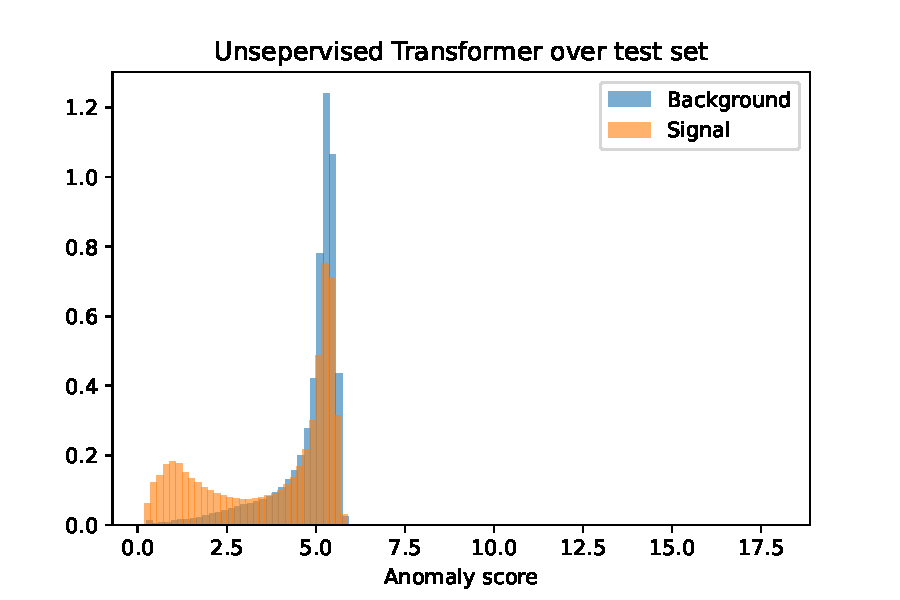
\includegraphics[width=2.5 in]{OLD/Images/Cap6/exampleAS.pdf}
  \caption{\centering Example of AS distribution plot. In this case we would have set the threshold around 3}
  \label{fig:exampleAS}
\end{minipage}%
\begin{minipage}{.5\textwidth}
  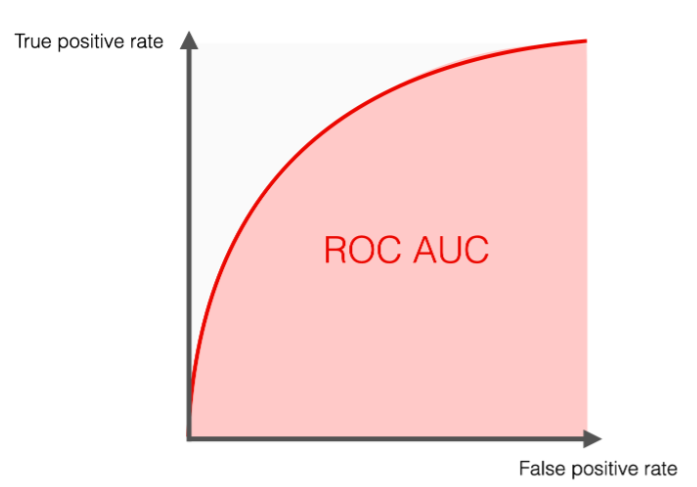
\includegraphics[width=2.5 in]{OLD/Images/Cap6/ROCAUC.png}
  \caption{ROC curve and AUC explained}
  \label{fig:exampleROCAUC}
\end{minipage}
\end{figure}


\noindent It is necessary to develop also a quantitative estimate of performance. We use the Area Under the Curve (AUC) \cite{AUC} and the Receiver Operating Characteristic (ROC) curve \cite{ROC}. They are computed starting from the confusion matrix, where four groups are presented to quantify misclassification errors: true positive (TP), true negative (TN), false positive (FP) and false negative (FN). From them we can calculate rates: 

\begin{equation}
    TPR=\frac{TP}{TP+FN}\ \rm , \ \rm \ \rm \ \rm \textit{FPR}=\frac{\textit{FP}}{\textit{TN+FP}}
\end{equation}
\\
\noindent where TPR is the True Positive Rate and FPR is the False Positive Rate. ROC curve, as shown in figure \ref{fig:exampleROCAUC}, is a plot showing the trade-off between TPR and FPR at various classification thresholds. The curve is always over the line where TPR=FPR and the closer it is to the top left corner, the better our model is learning. AUC is, as the name suggests, the area under the ROC curve; it is computed using an integration method, for instance the trapezoidal rule. A random classifier can only obtain a AUC=0.5 (TPR=FPR); a perfect classifier flies to a AUC=1.

%%%%%%%%%%%%%%%%%%%%%%%%%%%%
\section{Results}\label{sec:results}

As said in previous chapters, we need to optimize a few hyperparameters: learning rate $\eta$, number of heads in MHA $h$ and number of layers $L$. We execute the optimization training our model with different choices for these values and looking at the ones giving us the best results in terms of ROC and AUC. The best values we found during the training of the model are presented in table \ref{tab:results}, where "anti-$k_T$" stands for the not transformed dataset. 

\begin{table}[h!]
    \centering
    \begin{tabular}{|c||c|c|c||c|c|}
         \hline
         \rowcolor{lightgray}
         dataset & $\eta$ & $h$ & $L$ & best epoch & AUC\\
         \hline\hline
        anti-$k_T$ & $10^{-5}$ & 8  & 5 & 10 & 53\%\\
         \hline
        rotated & $10^{-6}$ &  8 & 32 & 27 & 66.4\% \\
         \hline
        transformed & $10^{-6}$ & 2 & 4 & 47 & 69.0\% \\
         \hline
    \end{tabular}
    \caption{\centering Results of our model training: best hyperparameters,\\ epoch for the best model and AUC}
    \label{tab:results}
\end{table}

\noindent Finally, results of our study are presented in figures below and then commented. 

\begin{figure}[h!]
\centering
\begin{minipage}{.5\textwidth}
  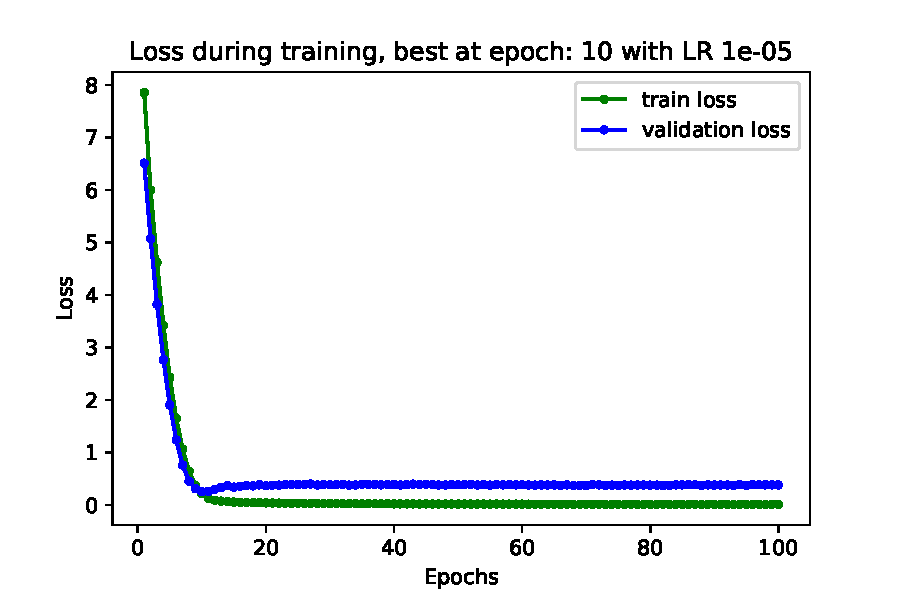
\includegraphics[width=3. in]{OLD/Images/Cap6/Results/KTTrainingLoopLossL5H8.pdf}
  \caption{Loss evolution, anti-$k_T$ dataset}
  \label{fig:KTTL}
\end{minipage}%
\begin{minipage}{.5\textwidth}
  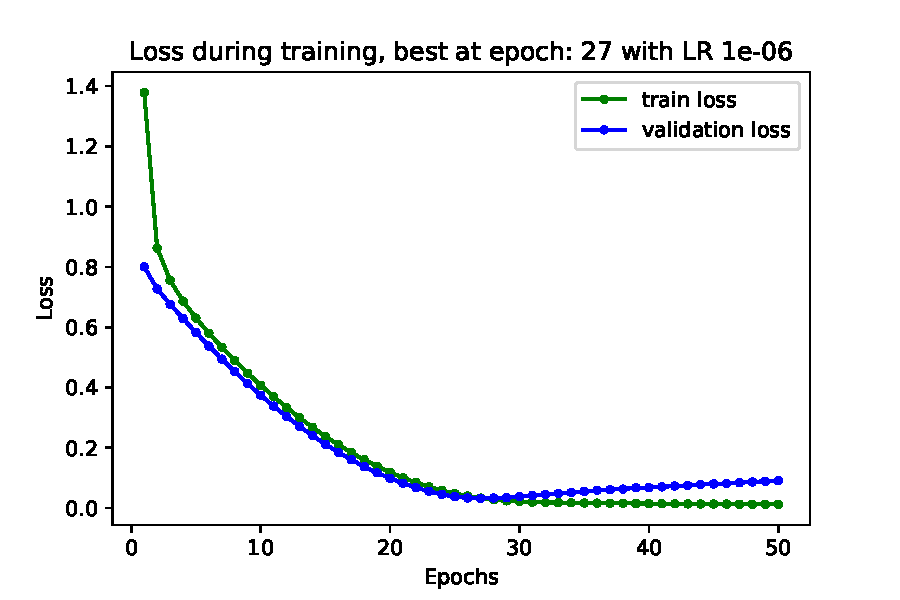
\includegraphics[width=3. in]{OLD/Images/Cap6/Results/ROTTrainingLoopLossL32H81e-06.pdf}
  \caption{Loss evolution, rotated dataset}
  \label{fig:ROTTL}
\end{minipage}
\begin{minipage}{.5\textwidth}
  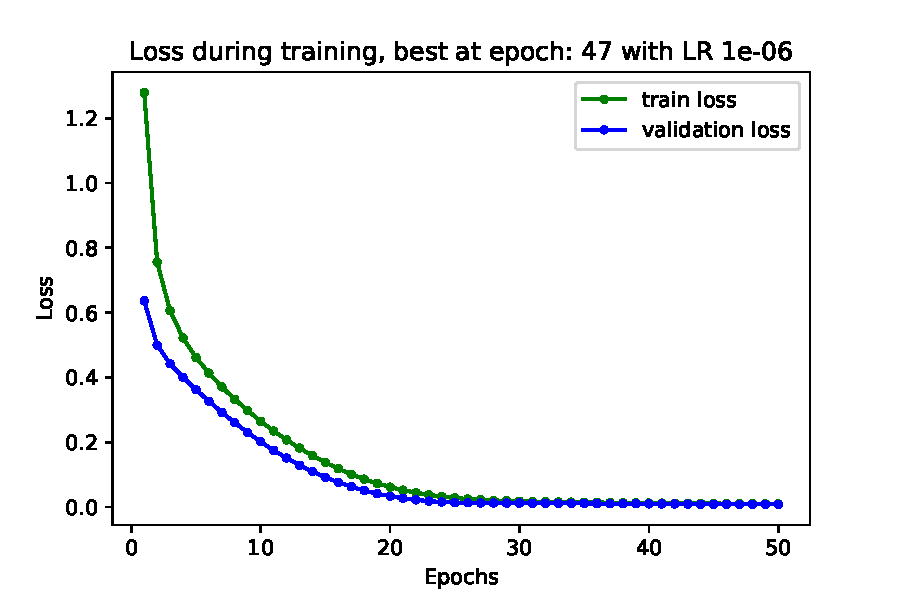
\includegraphics[width=2.7 in]{OLD/Images/Cap6/Results/TRANSFTrainingLoopLossL4H21e-06.pdf}
  \caption{Loss evolution, transformed dataset}
  \label{fig:TRTL}
\end{minipage}
\end{figure}

\begin{figure}[h!]
\centering
\begin{minipage}{.5\textwidth}
  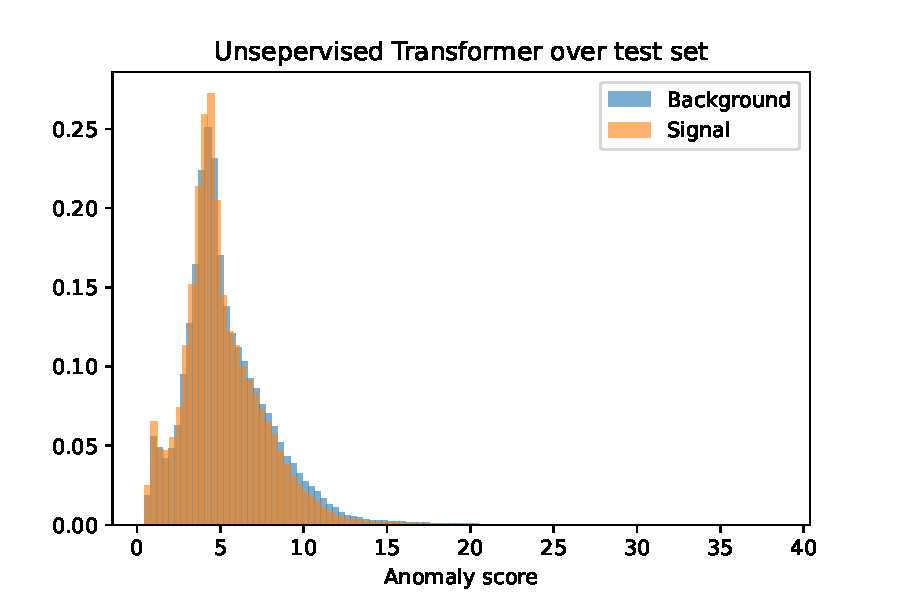
\includegraphics[width=3. in]{OLD/Images/Cap6/Results/KTAnomalyScore8H5.pdf}
  \caption{AS for the anti-$k_T$ dataset}
  \label{fig:KTAS}
\end{minipage}%
\begin{minipage}{.5\textwidth}
  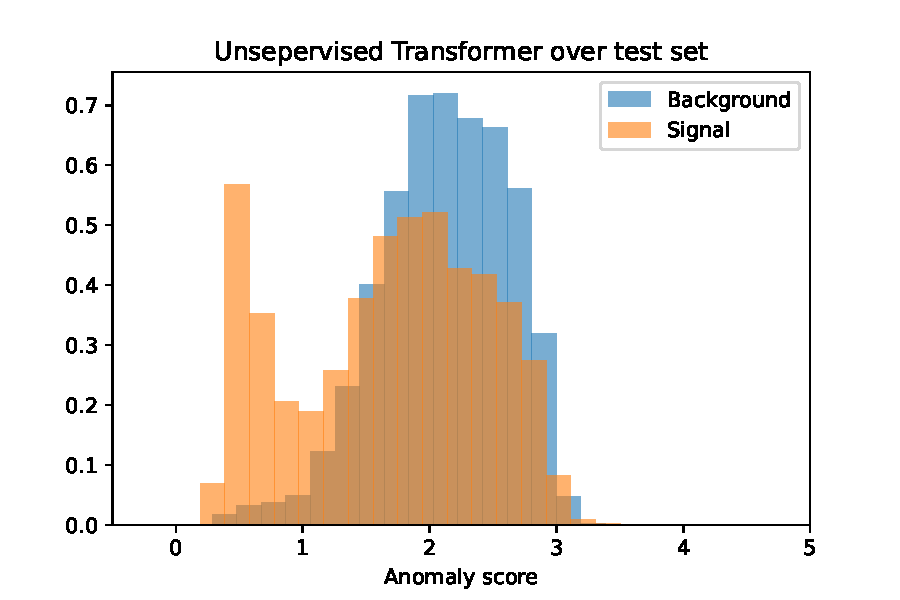
\includegraphics[width=3. in]{OLD/Images/Cap6/Results/ROTAnomalyScorezoom-6L32H8.pdf}
  \caption{AS for the rotated dataset}
  \label{fig:ROTAS}
\end{minipage}
\end{figure}

\begin{figure}[h!]
\centering
\begin{minipage}{.5\textwidth}
  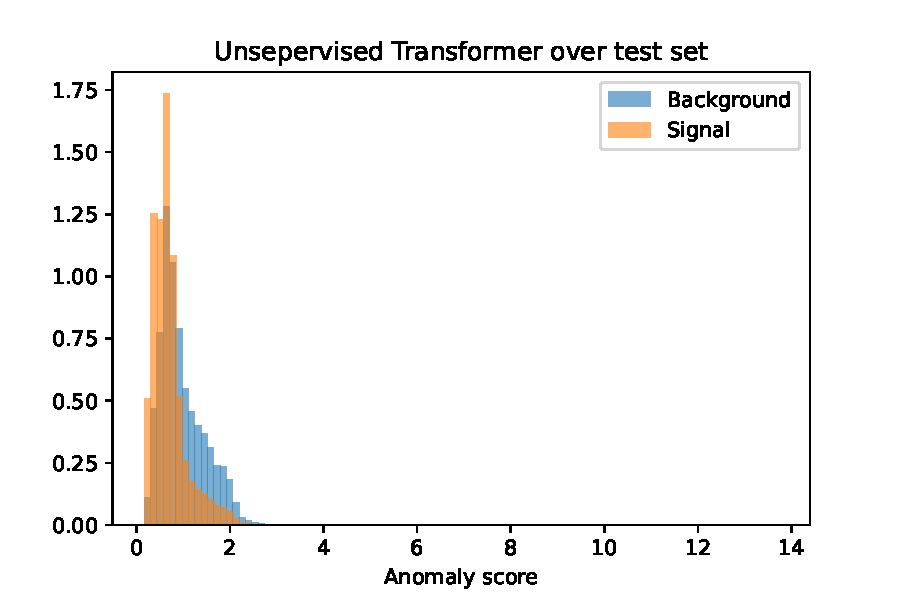
\includegraphics[width=3 in]{OLD/Images/Cap6/Results/TRANSFAnomalyScore4H21e-06.pdf}
  \caption{AS for the transformed dataset}
  \label{fig:TRAS}
\end{minipage}%
\begin{minipage}{.5\textwidth}
  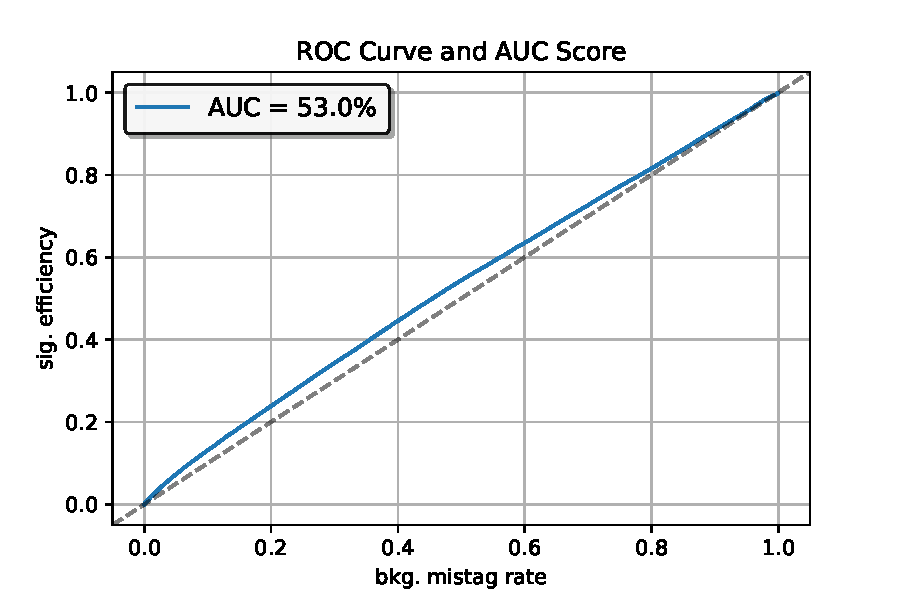
\includegraphics[width=3 in]{OLD/Images/Cap6/Results/KTAUCL5H8.pdf}
  \caption{AUC for the anti-$k_T$ dataset}
  \label{fig:KTAUC}
\end{minipage}
\end{figure}

\begin{figure}[h!]
\centering
\begin{minipage}{.5\textwidth}
  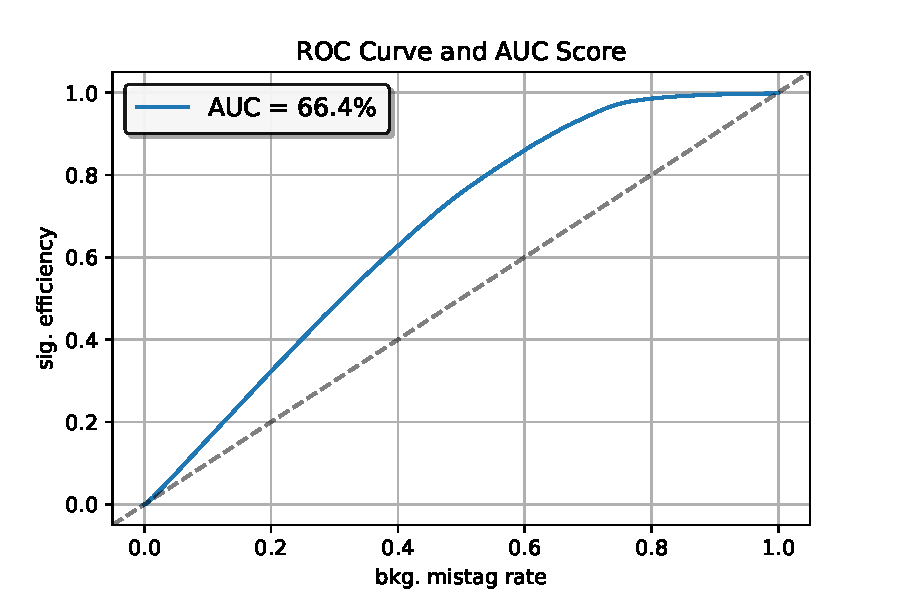
\includegraphics[width=3. in]{OLD/Images/Cap6/Results/ROTAUCL32H81e-06.pdf}
  \caption{AUC for the rotated dataset}
  \label{fig:ROTAUC}
\end{minipage}%
\begin{minipage}{.5\textwidth}
  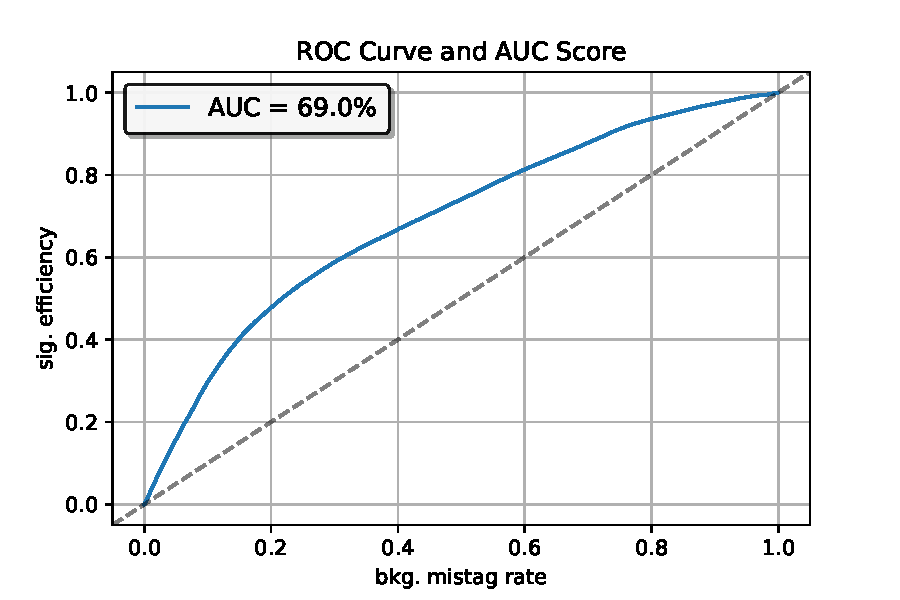
\includegraphics[width=3. in]{OLD/Images/Cap6/Results/TRANSFAUCL4H21e-06.pdf}
  \caption{AUC, transformed dataset}
  \label{fig:TRAUC}
\end{minipage}
\end{figure}

\noindent In figure \ref{fig:KTTL}, \ref{fig:ROTTL} and \ref{fig:TRTL} you can look at training plots showing the evolution of the MSE loss over training and validation set for each dataset; in figure \ref{fig:KTAS} , \ref{fig:ROTAS} and \ref{fig:TRAS} we present Anomaly Score distributions. In conclusion, in figure \ref{fig:KTAUC} , \ref{fig:ROTAUC} and \ref{fig:TRAUC} the ROC curve and the AUC plots are shown.\\
In all three cases, the MSE loss follows a reasonable evolution, with a minimum among chosen epochs. Given the presence of overfitting (values increasing after the minimum), a small number of training epochs (50) was chosen.\\
As clearly visible in figure \ref{fig:KTAS} and \ref{fig:KTAUC} where an AUC score of 53\% is presented (random classifier), if we train our model using data neither rotated nor transformed, we will not be able to distinguish between background and signal region. The reason behind this "failure" is the presence among data of jets with rotational symmetries, given the fact that for our purpose the position of the jet in the ($\eta , \phi $) plane is irrelevant. In fact, as discussed in paragraph \ref{sec:Transformation}, we assume that New Physics relies in the micro-structures of jets. If we do not transform the dataset, during the training phase, our model wastes time and data to learn that these jets are similar, resulting in a learning of only macro-structures of jets and a consequent inability to discriminate. Given the small deviation of anomalies from normal events, it is necessary that our model focuses on details.\\ 
As expected, rotated and transformed datasets obtain a higher value of AUC, respectively of 66.4\% and 69\%. Qualitatively speaking, AS plots show distributions distinguished between background and signal. Overall, we can notice that the transformed dataset performs better than the other; in fact, applying Lorentz boosts and frame change, all jets are pushed forward resulting in a smaller spatial aperture, because the new energy of jets $E_0$ is lower than original energy. If jets are pushed forward, they cover a smaller space in the ($\eta , \phi $) plan and for our model it is easier to learn to reconstruct background jets.\\
Anyway, in spite of the fact that we consider results acceptable for out project, it is important to note that perhaps the model we proposed and implemented is not the best choice for this task, given the not so high AUC score: the model can be optimized even more or we can choose another one.




